\documentclass[Main.tex]{subfiles}

\begin{document}

\section{Forze posizionali}
\toc

\subsection{Descrizione del problema}
Si intendono le forze della forma:
\begin{equation}
	f_{ij}=\varphi_{ij}(|x_i-x_j||) \frac{x_i-x_j}{|x_1-x_j|}
\end{equation}
Dove $\varphi_{ij}$ è lo scalare di forza che dipende dalla sola distanza dei due punti materiali e per il principio 3 vale che: $\varphi_{ij}=\varphi_{ji}$.

\begin{osservazione}  
	$\varphi_{ij}(r)$ è una funzione reale di variabile reale ($\geq 0$) e quindi esiste sempre una primitiva\footnote{vedi teorema fondamentale del calcolo integrale} rispetto alla variabile $r$. Tale primitiva viene chiamata energia potenziale associata alla forza in questione: \\
\begin{gather}
	\Phi_{ij} (r) = - \int \varphi_{ij} (r) dr \left( = -\int_A^B f_{ij} (s) \cdot ds \right) \\ \Rightarrow f_{ij} = - \frac{\partial}{\partial x_i} \Phi_{ij} (|x_i - x_j|)
\end{gather}
\end{osservazione}

\newpage
\begin{dm} \label{ammetteprimitiva}
	\begin{gather}
		- \pp{}{x}_{_i} \Phi_{ij} (|x_i - x_j|) = -\Phi_{ij}' (|x_i -x_j|) \frac{\partial}{\partial x}_{_i} |x_i -x_j|= \\
		- \Phi_{ij}' (|x_i - x_j|) \frac{\partial}{\partial x}_{_i} \underbrace{\sqrt{{(x_i - x_j) \cdot (x_i - x_j)}}}_{prodotto \ scalare} \\
		- \Phi_{ij}' (|x_i - x_j|) \frac{\frac{\partial}{\partial x}_{_i} (x_i \cdot x_i + x_j \cdot x_j -2x_i \cdot x_j)}{\ 2\sqrt{(x_i - x_j)\cdot (x_i - x_j)}}\end{gather} \begin{gather}
		- \Phi_{ij}' (|x_i - x_j|) \frac{\cancel{2} x_i - \cancel{2}x_j}{\cancel{2} |x_i - x_j|} \\
		- \Phi_{ij}' (|x_i - x_j|) \frac{x_i - x_j}{|x_i - x_j|} = \varphi (|x_i - x_j|)\frac{x_i - x_j}{|x_i - x_j|} 
	\end{gather}
\end{dm}


Questo tipo di forze, dette anche \textit{centrali}, sono quelle presenti tra i punti del sistema isolato (forze interne).

\newpage
\subsection{Conservazione del momento angolare}
\noindent Cruciale per lo studio di forze posizionali è il momento angolare
\begin{df}[Momento angolare]
	$\ell := x \times m \dot x$
\end{df}
Adesso utilizzando il momento angolare appena definito ha senso riprendere l'esempio dell'oscillatore armonico per mostrare alcune leggi di conservazione.

\begin{tema}[Oscillatore armonico spaziale] 
\begin{equation}\notag
	m \ddot x = -kx\longrightarrow \boxed{ \ddot x=-\omega^2 x\Rightarrow x(t)=a \cos(\omega t) + b \sin(\omega t)} 
\end{equation}
	Con $x, \ a, \ b \ \in \Rr^3$. Utilizzando la definizione di momento angolare $\ell$ il cui modulo è $|\ell|=|x||p|\sin \theta$ si osserva che se la sua derivata si annulla allora è una quantità conservata, quindi $\ell(t)=\ell(0) \ \forall t$. Questo è verificato per l'oscillatore armonico:
	\begin{equation}\notag
		\dot \ell = \dd{\ell}{t}= \dd{}{t}\left(x \times m \dot x\right) = \underbrace{\dot x \times m \dot x}_{\dot x \parallel \dot x \Rightarrow=0} + x \times m \ddot x = \underbrace{x \times (-k x)}_{x \parallel x \Rightarrow=0}=0
	\end{equation}
	Segue che se $\dot \ell(t)=0 \Rightarrow \ell(t)= \ell(0)= x(0) \times -kx(0)$. Esistono due possibilità:
	\begin{enumerate}
		\item $\dot \ell(0)=0 \Rightarrow x(0) \parallel \dot x(0) \Rightarrow x(t) \parallel \dot x(t) \ \forall t$
		\item $\dot \ell (0) \neq 0 \Rightarrow x(t) \notparallel \dot x(t) \ \forall t$
	\end{enumerate} 	
	Da queste considerazioni segue che 
\begin{equation}\label{orbitapiana} \notag
 	x(t) \cdot \ell(t) = 0 \ \forall t \Rightarrow x(0) \cdot \ell(0)=0= \boxed{x_1 \ell_1+x_2+\ell_2+x_3\ell_3=0}
 \end{equation}
Che è l'equazione di un piano perpendicolare a $\ell$ passante per l'origine. Questo implica che il moto dell'oscillatore armonico tridimensionale è piano, il piano è quello dell'equazione \eqref{orbitapiana}.

Adesso ha senso chiedersi, data la soluzione del problema:
\begin{equation}
	\begin{cases}
		x_1(t) = a_1 \cos ( \omega t ) + b_1 \sin (\omega t) \\
		x_2 (t) = a_2 \cos ( \omega t) + b_2 \sin (\omega t)
	\end{cases}
\end{equation}
Qual è la forma dell'orbita $\gamma:t \rightarrow \left( \begin{array}{c} x_1(t) \\ x_2(t) \end{array} \right)$?

Osservando che $a_1 \cos ( \theta ) + b_1 \sin ( \theta) = A \cos ( \theta + \alpha )$ 
con $\tan(\alpha) =- \frac{b_1}{a_1}$. Allora
\begin{equation}
	\begin{cases}
		x_1(t) = A \cos (\theta + \alpha) = A \cos(\omega t + \alpha)\\
		x_2(t) = B \cos( \omega t + \beta) 
	\end{cases}
\end{equation}
Si definisce ora: $\psi := \omega t+ \alpha$ e $\delta :=\beta - \alpha$.
\begin{equation}
	\begin{cases}
		x_1(t) = A \cos( \psi)\\
		x_2(t) = B \sin ( \psi + \delta)
	\end{cases} 
\end{equation}
Dalla prima si trova $
	\boxed{
 \frac{x_1}{A} = \cos ( \psi)}$
e  dalla seconda 
\begin{equation}\notag
	 \frac{x_2}{B} = \cos \beta \cos \delta - \sin \psi \sin \delta\Rightarrow \boxed{\sin \psi = \left (- \frac{x_2}{B} + \frac{x_1}{A} \cos \delta \right)}
\end{equation}
Sfruttando l'identità trigonometrica $\sin^2 \psi + \cos^2 \psi = 1$ 
\begin{equation}
	\frac{x_1^2}{A^2} + \frac{1}{\sin^2 \delta} \left( \frac{x_1}{A} \cos \delta - \frac{x_2}{B} \right)^2=1
\end{equation}
Questa è l'equazione di una conica. In particolare è l'equazione di un'ellisse ruotata:
\begin{equation}
	\frac{x_1^2}{A^2} + \frac{x_2}{B^2} - \frac{2x_1x_2}{AB} \cos \delta= \sin^2 \delta
\end{equation}
Questo problema può essere posto anche in forma matriciale:
\begin{equation}\label{=1} \notag
	\left (x_1 \ x_2 \right) \underbrace{\left( \begin{matrix} \frac{1}{A^2 \sin^2 \delta} & - \frac{\cos \delta}{AB \sin ^2 \delta} \\ - \frac{ \cos \delta}{ AB \sin^2 \delta} & \frac{1}{B^2 \sin^2 \delta} \end{matrix} \right)}_{M} \left( \begin{array}{c} x_1 \\ x_2 \end{array} \right)=1
\end{equation}
$M$ è una matrice simmetrica perchè è associato a una forma bilineare che rappresenta una conica. Allora vale che $M^T=M$, allora per il teorema spettrale $\exists R$, \\ ($R^TR=\1 \iff R$ è ortogonale), $:R^TMR = \left( \begin{matrix} m_1 & 0 \\ 0 & m_2\end{matrix}\right)$ con $m_1, \ m_2  \in \Rr$ sempre per il teorema spettrale. È possibile scrivere una forma canonica di questa relazione. Siano $x \in \Rr^2$ i vettori di $S''$ e $y \in \Rr^2$ i vettori di $S$. Sfruttando la \eqref{=1} si ha:
\begin{equation}
	\begin{split}
	x=Ry &\Rightarrow (Ry)^TM(Ry)=1\Longrightarrow x^TMx=1\\
	&=y^T\underbrace{R^TMR}_{\in D^{2 \times 2}}y = 1 = \left( y_1 \ y_2 \right) \left( \begin{matrix}
 m_1 & 0 \\ 0 & m_2 	
 \end{matrix} \right) \left( \begin{array}{c} y_1 \\ y_2 \end{array} \right)\\
 &\Rightarrow \boxed{ m_1 y_1^2 + m_2 y_2^2 =1}
\end{split}
\end{equation}
Si può dimostrare che $m_1$ e $m_2$ esistono sempre:
\begin{gather}
		\det (m- \lambda \1 ) =0 \iff \lambda^2 - tr(M) \lambda + \det M= 0 \notag \\ \notag
		\iff \lambda^2 + \frac{1}{A^2B^2 \sin^4 \delta} - \frac{ \cos^2 \delta}{A^2B^2 \sin^4 \delta } - \left( \frac{1}{A^2} + \frac{1}{B^2} \right) \frac{\lambda}{\sin^2 \delta} =0\\ \notag
		\lambda_\pm = \frac{1}{2} \left[ \underbrace{\left( \frac{1}{A^2}+ \frac{1}{B^2} \right) \frac{1}{\sin^4\delta}}_{\tau >0} \pm \sqrt{ \left( \frac{1}{A^2}+\frac{1}{B^2} \right)^2 \frac{1}{\sin^4 \delta} - \frac{4}{\underbrace{A^2B^2 \sin^2 \delta}_{\gamma >0} }}\right]
\end{gather}
Se $\lambda_\pm$ esistono devono essere positivi enndendo che $\tau > \tau \sqrt{ 1 - \frac{\gamma}{\tau^2}}$ con $\gamma, \ \tau  >0$. La matrice $M$ e la conica ad essa associata sono definite positive.
\begin{gather}
\notag \Rightarrow \exists \  \lambda_\pm \in \Rr \iff \left( \frac{1}{A^2} + \frac{1}{B^2} \right)^2 \frac{1}{\sin^4 \delta} - \frac{4}{A^2 B^2 \sin ^2 \delta}  \geq 0	\\ \notag
\iff  \frac{1}{A^4 sin^4 \delta} + \frac{1}{B^2 \sin^4 \delta} + \frac{2}{A^2B^2 \sin ^4 \delta } - \frac{4}{A^2 B^2 \sin^2 \delta} + \\  \notag + \underbrace{\frac{2}{A^2B^2 \sin^4 \delta}- \frac{2}{A^2B^2 \sin^4 \delta}}_{+0} \geq 0\\
\iff \left( \frac{1}{A^2} - \frac{1}{B^2} \right)^2 \frac{1}{\sin^4 \delta} + \frac{4}{A^2 B^2 \sin ^4 \delta } \left( 1- \sin^2 \delta \right) >0 \notag
\end{gather}
La disuguaglianza è sempre verifica e, come prevedeva il teorema spettrale, $\lambda_\pm$ esistono sempre e i semiassi dell'ellisse sono $a= \frac{1}{\sqrt{\lambda_-}}$ e $b=\frac{1}{\sqrt{\lambda_+}}$.
\begin{osservazioni}
	\item per $\delta=0$ l'equazione diventa $\frac{x_1^2}{A^2} + \frac{x_1}{B^2} \boxed{-} \frac{2x_1x_2}{AB} = \left( \frac{x_1}{A} \boxed{-} \frac{x_2}{B} \right)^2= \iff x_1 = \frac{B}{A}x_1$
	\item per $\delta = \pi$ si ha invece $\frac{x_1^2}{A^2} + \frac{x_1}{B^2} \boxed{+} \frac{2x_1x_2}{AB} = \left( \frac{x_1}{A} \boxed{+} \frac{x_2}{B} \right)^2= \iff x_1 = -\frac{B}{A}x_1$
\end{osservazioni}
\end{tema}

\newpage
\noindent Visto questo esempio si può generalizzare la \underline{conservazione del} \underline{momento angolare}:
\begin{df}[Momento della forza]
	$\ell=x(t) \times m\dot x (t)$ 
	
	$\Rightarrow \boxed{\dot \ell =x(t) \times m \ddot x(t) = x(t) \times f}$
\end{df}
Si vede subito che $\dot \ell=0 \iff x \parallel f$. Essendo il momento della forza derivata del momento angolare quando il primo è nullo il secondo si conserva. Inoltre per la definizione di forza tali per cui $f \parallel x$ (perchè $f= \varphi \hat x$) si può concludere che in un campo di forze centrali $\dot \ell=0 \Rightarrow \ell$ è conservato.
\begin{osservazione}
	Una delle conseguenze di quest'ultima conclusione è che quando un corpo è in moto in un campo di forza centrale la sua velocità areolare è constante.
	
	\begin{dm}
	\vspace{-10pt}
	\begin{figure}[H]
		\center 
		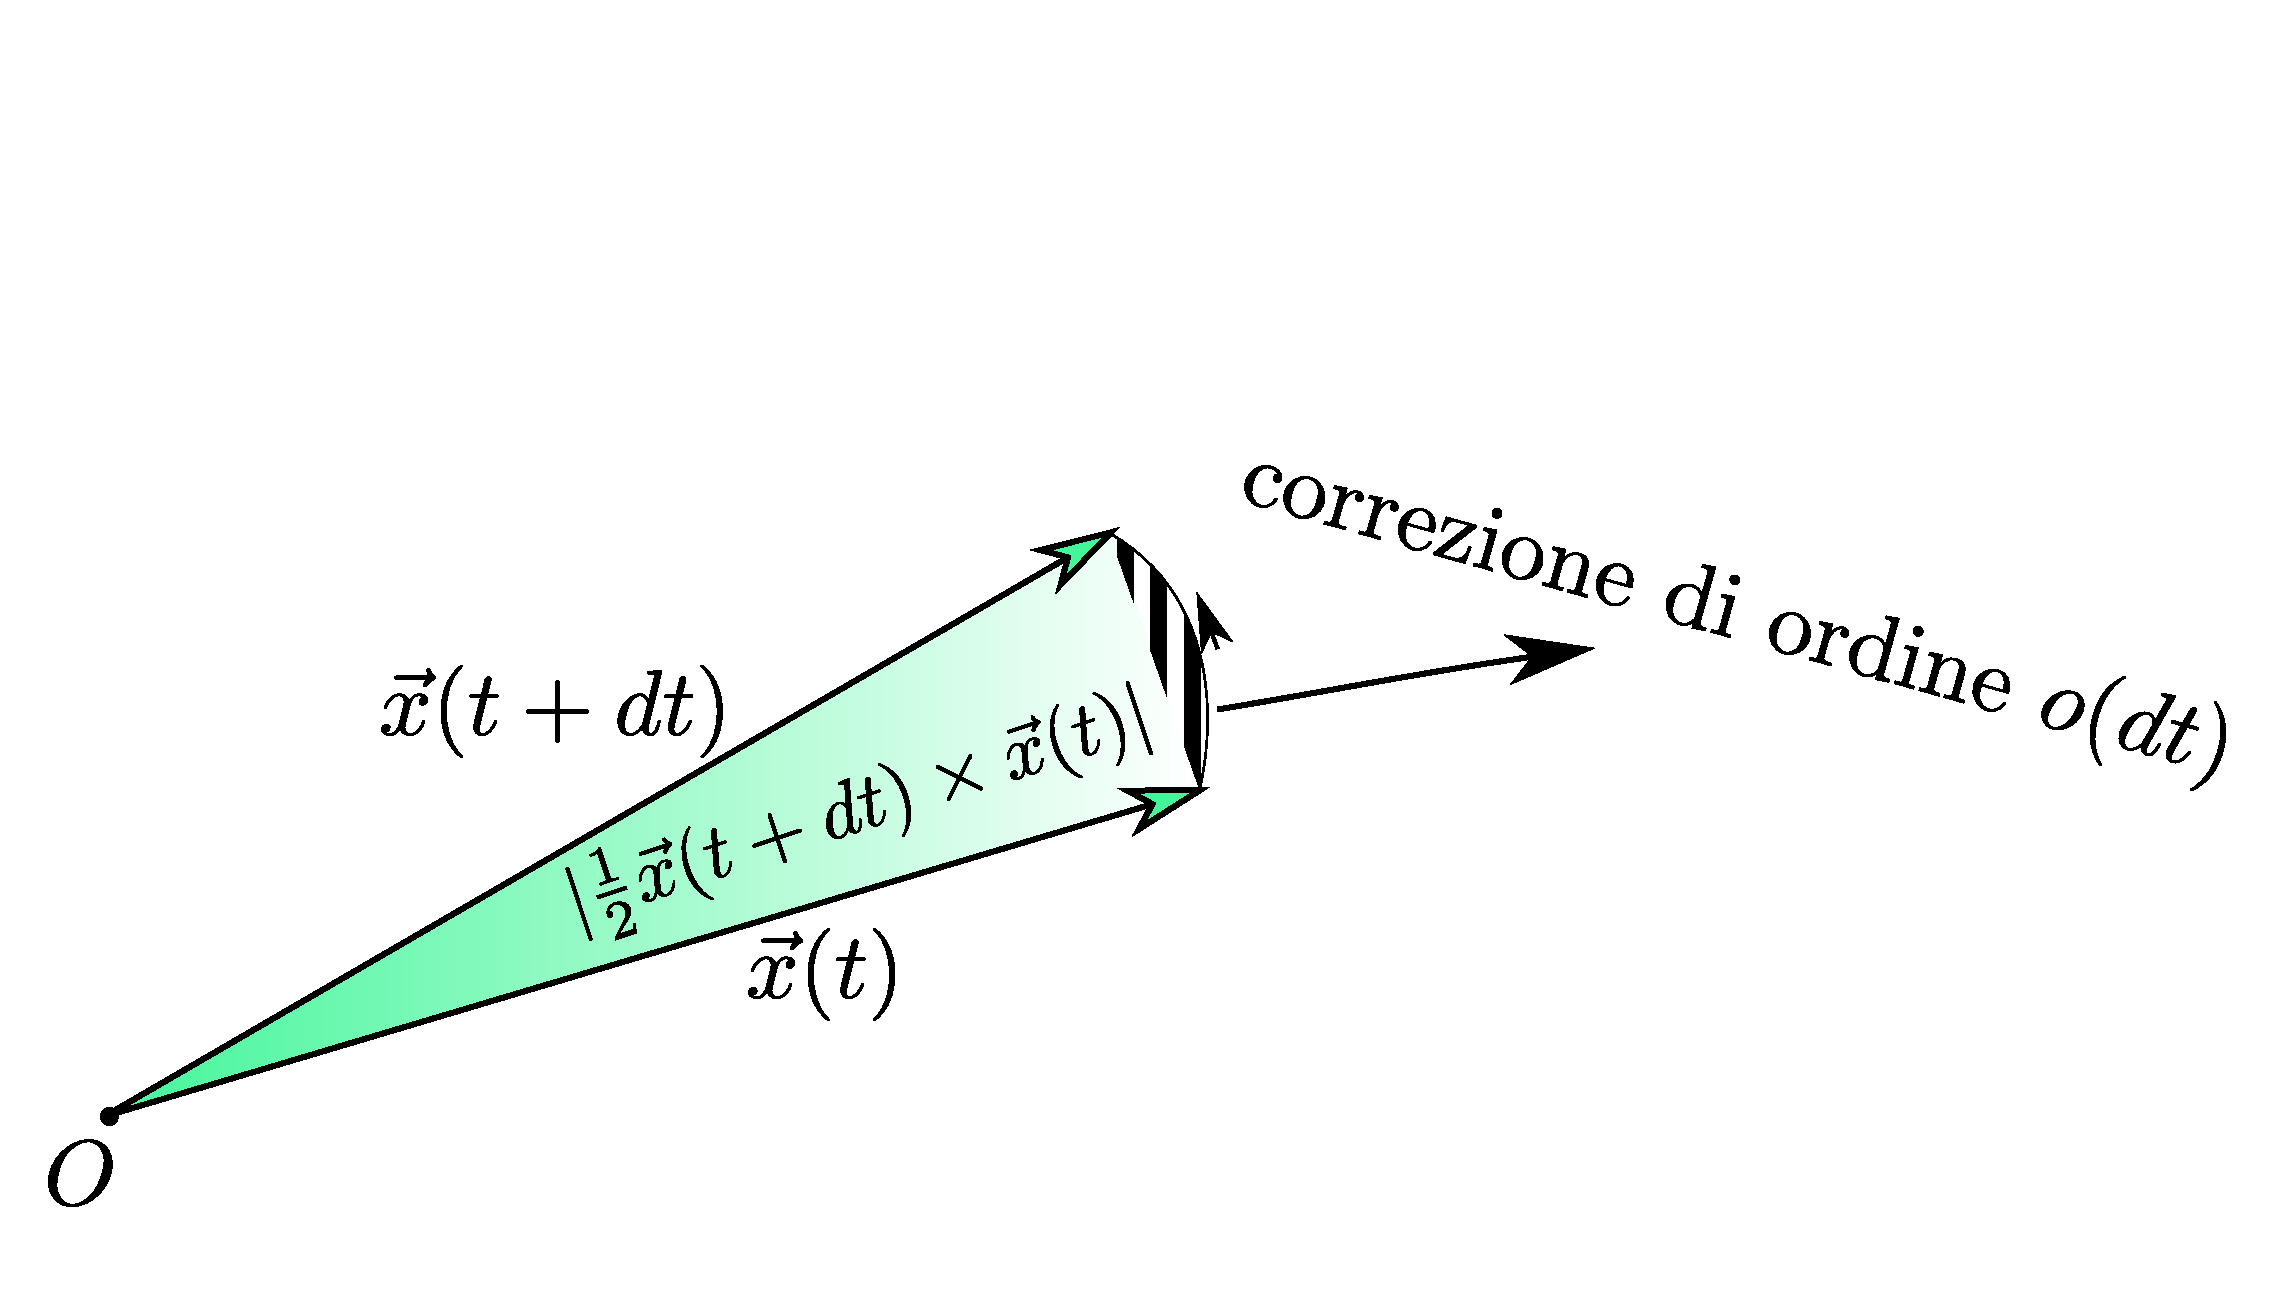
\includegraphics[width=0.7\textwidth]{images/kepler.pdf}
	\end{figure}

 	Per definizione geometrica la velocità areolare:
 	\begin{gather}
 		\Delta A(t) = \frac{|x(t) \times x(t+dt)|}{2}=\\
 		=\frac{1}{2} \left| x(t) \times \left( \cancel{x(t)} + \dot x(t) \Delta t + o(\Delta t^2)\right)\right|=\\
 		=\frac{\Delta t}{2m} \left| \ell(t) + o(\Delta t) \right|
 	\end{gather}
 	\begin{gather}
 		\Rightarrow \dot A(t) = \lim_{\Delta t \rightarrow 0} \frac{\Delta A}{\Delta t} = \frac{| \ell(0)|}{2m} = \text{cost}
 	\end{gather}
	\end{dm}
\end{osservazione}


\subsection{Forza di gravitazione}
\begin{equation}
	F_{ij}=-G \frac{m_im_j}{(x_i-x_j)^2} \hat x_{ij} \notag
\end{equation}
La forza gravitazionale, a differenza di quella di interazione elettrica, prevede l'esistenza soltanto di massa positiva e  quindi è solo attrattiva.
Le caratteristiche legate alla gravitazione newtoniana sono descritte dalle:

\noindent
\subsubsection{Leggi di Keplero}
\begin{enumerate}
	\item I pianeti si muovo su orbite ellittiche in cui il sole occupa uno dei due fuochi\footnote{È corretta solo per certe approssimazioni, in realtà i pianeti non compiono vere e proprie orbite ellittiche a causa delle pertubazioni gravitazionali dovute agli altri pianeti.}.
	\item La velocità aerolare è costante.
	\item $\frac{T^2}{a^3}=cost$, essendo $T$ il tempo di rivoluzione e $a$ il semiasse maggiore dell'orbita ellittica. 
\end{enumerate}

Perché la gravitazione ha questa forma? Un po' è stato già discusso prima, cioè che le forze fondamentali sono di fatto forze centrali. Di seguito è spiegato perché la forma risulta di questo tipo:
\begin{itemize}
	\item \textbf{Perché il prodotto tra le masse?} Una delle grandi conquiste di Newton è stata quella di notare che le forze celesti e quelle terrestri sono le stesse (in contrapposizione alla fisica aristotelica). E sulla terra tutti i corpi cadono con accelerazione costante e quindi vale:
	$$
	a=\text{cost.}=\frac{F_g}{m}
	$$
	ma ci è possibile se e solo se $F_g \propto m$. Ovviamente la forza dipende anche dalla massa della Terra che attrae il corpo, quindi $F \propto m_1 m_2$;
	\item \textbf{Perché dipende dall'inverso del quadrato di r?} Si può giustificare in vari modi (per esempio flusso), ma uno dei più importanti, che è quello che riporta Newton, usa l'invarianza di scala $\frac{T^2}{r^3}=\text{cost.}$ proposta da Keplero osservando il sistema solare.

\end{itemize}

\begin{dm}
	Prendendo un sdr inerziale solidale con il sole di massa $M$ si ha:

	\begin{equation}
		m \frac{d^2}{dt^2} x = -Gm M \varphi (|x|) \hat x
	\end{equation}

	Si può riscalare posizione e tempo come $ \begin{cases}
	 x=a x' \\
	 t= Tt'
	 \end{cases}$

	\begin{equation}
		\frac{a}{T^2} \frac{d^2x'}{dt'^2} = GM \varphi (a |x'|) \hat x'
	\end{equation}

	moltiplicando per $a^2$

	\begin{equation}
		\frac{a^3}{T^2} \frac{d^2x'}{dt'^2} = GM a^2 \varphi (a |x'|) \hat x'
	\end{equation}

	C'è così  un riscalamento, quindi le orbite si riducono a una sola e il periodo di rivoluzione diventa unico. Nell'equazione per Keplero $\frac{a^3}{T^2}=\text{costante}$

	\begin{equation}
		\frac{a^3}{T^2} = k \longrightarrow \frac{d^2x'}{dt'^2} = ( \frac{1}{k} GM) \varphi(a|x'|) \hat x'
	\end{equation}

	se $a^2 \varphi (a |x'|) = \varphi(|x'|) \Longleftrightarrow \varphi(a|x'|) = a^{-2} \varphi(|x'|)$. Cioè $\varphi$ è omogenea di grado -2 in $x'$ e quindi, come dimostriamo sotto, è uguale a $\frac{1}{x^2}$

\end{dm}



\begin{df}[Funzione omogenea]
	Una funzione $f : \mathbb{R}^d \rightarrow \mathbb{R}$ si dice omogenea di grado $s \in \mathbb{R}$ se $f(\lambda x) =
\lambda^s f(x)$ per qualsiasi $\lambda > 0$.
\end{df}

\begin{teo}[Teorema di Eulero per funzioni omogenee]
Se f è $C^1$ e omogenea di grado s, allora vale che
\begin{equation}
	x \cdot \nabla f(x) = s f(x)
\end{equation}
con $x \in \R^d$.In particolare se $d=1$ , $f(x) = c|x|^s$, dove c è una costante.
\end{teo}


\begin{dm}
Derivando rispetto a $\lambda$ e si pone $\lambda=1$
\begin{gather*}\notag
	\left. \frac{d f(\lambda x)}{d\lambda}\right|_{\lambda=1} = \left. \frac{d f(\lambda x)}{d \lambda x} \cdot x \right|_{\lambda=1} = \\ =x_1 \frac{d f(x)}{dx_1} + ... + x_d \frac{f(x)}{dx_d}=\nabla f(x) \cdot x
\end{gather*} 
I precedenti sono solo identità, valide per ogni funzione.
\begin{gather}
	\left. \frac{d f(\lambda x)}{d\lambda} \right|_{\lambda=1} = \left. \frac{d \lambda^s f(x)}{d\lambda}\right|_{\lambda=1} =\\ = \left. f(x) \left. \frac{d \lambda^s}{d\lambda} \right|_{\lambda=1}= f(x) s \lambda^{s-1} \right|_{\lambda=1}=s f(x)
\end{gather}

dove si è usato l'omogeneità della $f$ rispetto alle $x$. Così si conclude la dimostrazione della prima parte dell'enunciato. \\

Per la seconda parte si nota che per per d=1 il teorema di Eulero afferma che $xf' (x) = s f(x)$ che è un'equazione differenziale del primo ordine a variabili separabili.
Verificata $\iff  x\frac{d}{dx}f = sf \iff \frac{df}{f} = s \frac{dx}{x}$
\begin{gather}\notag
	\int \frac{df}{f} = s \int \frac{dx}{x} \iff ln|f| = s \cdot ln|x| + c
\\ \notag
	ln |f| - ln |x| ^ s = c \iff ln \frac{|f|}{|x|^s}= c \iff |f| = e^c |x|^s
\\
	f(x) = c |x|^s
\end{gather}

Quindi per il teorema di Eulero nel caso gravitazionale precedente dove $s=-2$ e $d=1$, abbiamo $\varphi(r) = \frac{c}{r^2}$ e scegliamo c=1 (abbiamo già tirato fuori la $G$ da questa costante $c$).
\end{dm}

\begin{osservazione}
Per $d=2$ sia $f(x,y) = \frac{1}{x^2+y^2}$ $\hat f (x,y) = \frac{x}{(x^2+y^2)^{3/2}}$ sono omogenee di grado $-2$ e sono profondamente diverse. Quindi soltanto per $d=1$ esiste una sola forma analitica per le funzioni omogenee.
\end{osservazione}

\newpage
\subsubsection{Validità dell'approssimazione di massa puntiforme}
Ha senso chiedersi adesso se \emph{la forza a distanza è la stessa che si avrebbe se la massa della terra fosse concentrata tutta nel suo centro.} 

\begin{wrapfigure}{l}{0.35\textwidth}
	\includegraphics[width=0.4\textwidth]{images/sferam.pdf}
\end{wrapfigure}
\noindent Si ipotizza innanzitutto che:
\begin{itemize}
	\item la densità di massa $\M$ sia $\rho(s)$ dove $s$ è la distaza tra il punto della sfera considerata e il suo centro ($s=|\overline{OP_i}|$)
	\item per simmetria sferica tutti i contributi non paralleli all'asse z si elidono a vicenda
\end{itemize}
La componente $z$ della forza (per unità di volume) esercitata da $P_i$ su $m$ vale 
\begin{equation}
	\F = - \frac{Gm \rho(s) cos \gamma}{d^2}
\end{equation}
\newline \ \newline 

Per calcolare la forza complessiva sarà necessario integrare quest'ultima su tutto il volume della sfera.
\begin{gather}
	\begin{cases}
		r= s\cos \theta + d \cos \gamma \\ 
		s \sin \theta = d \sin \gamma 
	\end{cases} \Rightarrow \begin{cases}
 	d \cos \gamma = r - s \cos \theta \\ d \sin \gamma = s \sin \theta 
 \end{cases}  \\ \iff \begin{cases}
 	d^2=r^2 + s^2 -2r s \cos \theta \\ \cos \gamma = \frac{r- s \cos \theta}{d}
 \end{cases}
\end{gather}
Si può ora riformulare l'espressione di $\F$ nel seguente modo:
\begin{equation}
	\F = -G \rho (s) m \frac{r - s \cos \theta}{[ r^2 + s^2 -2rs \cos \theta ]^{3/2}}
\end{equation}
Per $r > R_T$
\begin{gather}
	\F = -G m \int_{\S} \frac{\cos \gamma \rho (s)}{d^2} d^3s = \\ =Gm \int_0^{2\pi} d \varphi \int_0^\pi d \theta \int _0^R ds \rho(s) 	\frac{(r- s \cos(\theta)) s^2 \sin \theta}{(r^2 +s^2 -2rs \cos \theta)^{3/2}}= \notag\\ =Gm 2 \pi \int_0^\pi d \theta \int_0^R ds \rho(s) \pp{}{r} (r^2 + s^2 -2rs \cos \theta )^{-1/2} \\ \boxed{\int d\theta , \int ds\text{ non dipendono da $r$}}\\
	=\pp{}{r} Gm 2 \pi \int_0^\pi d \theta \int_0 ^R ds \frac{s^2 \rho(s) \sin \theta}{ \sqrt{r^2 + s^2 -2rs \cos \theta}}
\end{gather}
Cambio di variabile $u=-cos \theta \Rightarrow du = \sin \theta d \theta \Rightarrow-1\leq u \leq 1$
\begin{gather}
	\F = \pp{}{r} \left[ 2 \pi Gm \int_0^R ds \int_{-1}^{1} \frac{ \rho(s) s^2}{\sqrt{r^2 + s^2 + 2r  s u}} du \right] =  \\
	= \pp{}{r} \left[ Gm 2 \pi \int_0^R ds \rho(s)  \frac{s^2}{rs} \sqrt{r^2 + s^2 + 2rsu} \left.  \right] \right|_{u=-1}^{u=1}=\\
	= \pp{}{r} \left[ Gm 2 \pi \int_0^R ds \rho(s) \frac{s}{r}[( r + s) -(r-s)] \right]= \\
	=\pp{}{r} \left[\frac{4 \pi Gm}{r} \int_0^R ds \rho (s) s^2 \right]= -\frac{Gm}{r^2} \left( 4 \pi \int_0^R ds \rho(s) s^2\right)= \notag \\ =\boxed{- \frac{GmM}{r^2}} 
\end{gather}

La risposta quindi è si, per $r>R_T$ nell'approssimazione di terra sferica, è possibile utilizzare l'approssimazione di punto materiale posto al centro della sfera la cui massa è quella della terra. Trattandosi di un punto materiale il caso in considerazione è discreto:
\begin{equation}
	\begin{cases}
		\F_{d} = -Gm \sum_{p} \frac{m_p(x-y_p)}{|x-y_p|^3}\\
		\F_{c}=-Gm \int \frac{\rho(s) (x-y)}{|x-y|^3}d^3y
	\end{cases}
\end{equation}

È possibile passare dal continuo al discreto tramite la funzione delta di Dirac ponendo $\rho(y)= \sum_p m_p \delta (y- x_p)$. Nella trattazione appena fatta si è implicitamente utilizzato che $\rho(y) = \rho(|y|)$. Ammesso che $\rho$ non dipenda esclusivamente dal modulo di $y$ si procede sviluppando il potenziale gravitazionale:

\begin{comment}
\begin{gather}
	U(x):= - Gm \int \frac{\rho(y) d^3y }{|x-y|}= \\\overset{|x| \gg 1}{\overset{\downarrow}{=}} -Gm \left[ \frac{\int \rho(s) d^3y}{|x|} + \underbrace{\frac{1}{|x|^2} \int \rho(y) ( y \cdot \hat x) d^3y}_{\text{dipolo}} + \underbrace{\frac{1}{|x|^3} \int \rho(y) \frac{3 ( y \cdot \hat x)^2 - |y|^2}{2} d^3y}_{\text{quadrupolo}} + O\left( \frac{1}{|x|^4} \right) \right]
\end{gather}
\end{comment}

\begin{gather}
	U(x):= - Gm \int \frac{\rho(y) d^3y }{|x-y|}= \\ \notag
	\resizebox{1\textwidth}{!}{$ \overset{|x| \gg 1}{\overset{\downarrow}{=}} -Gm \left[ \frac{\int \rho(s) d^3y}{|x|} + \underbrace{\frac{1}{|x|^2} \int \rho(y) ( y \cdot \hat x) d^3y}_{\text{dipolo}}  +  +\underbrace{\frac{1}{|x|^3} \int \rho(y) \frac{3 ( y \cdot \hat x)^2 - |y|^2}{2} d^3y}_{\text{quadrupolo}} + O\left( \frac{1}{|x|^4} \right) \right]$}
\end{gather}
Il termine di dipolo si può riscrivere come:
\begin{equation}
	-Gm \frac{1}{|x|^2} \int \rho(y) (y \cdot \hat x) d^3 y = -Gm \frac{x}{|x|^3} \cdot \underbrace{\left( \int \rho (y) y d^3 y \right)}_{\propto \text{ centro di massa}}
\end{equation}
\begin{equation}
	=- Gm \underbrace{\left( \int \rho(y) d^3 y \right)}_{\text{Massa della distribuzione}} \frac{x}{|x|^3} \cdot X
\end{equation}
Con $X:= \frac{\int \rho(y) y d^3y}{\int \rho(y) d^3y}$ ma se si sceglie un sistema di coordinate con origine nel centro di massa allora $X=0$ e quindi anche il termine di dipolo. Per la prima equazione cardinale della dinamica la risultante delle forze esterne è uguale alla massa totale per l'accelerazione del centro di massa. Essendo le forze esterne nulle allora il centro di massa si muove di moto rettilineo uniforme, quindi per il principio della relatività di Galileo esiste un sistema di riferimento inerziale per cui $X=0 \ \underline{\forall t}$. 

\begin{osservazione}
Nel caso dell'elettrostatica $\rho$ assume il senso della \emph{densità di carica}, a differenza del potenziale gravitazionale il la correzione di dipolo non si può annullare, mettendosi in un sistema di riferimento opportuno con una trasformazione di coordinate, perchè il \emph{centro di carica} non soddisfa la stessa proprietà del baricentro.
\end{osservazione}

\newpage
\subsection{Forza elastica}
\begin{equation}
	\varphi_{ij}=-k_{ij}|x_i-x_j| \notag
\end{equation}
Viene detta anche legge di Hooke ed è una forza di carattere fenomenologico (ha cause più fondamentali e l'equazione citata sopra può essere derivata da equazioni più fondamentali della natura). Quello scritto sopra è il modulo (con segno) della forza, invece $F$ è:
\begin{equation}
	F_{ij}=-k_{ij}(x_i-x_j) \notag
\end{equation}
$k$ può essere positivo (forza repulsiva) o negativo (forza attrattiva).

\end{document}